  \documentclass{beamer}
\usepackage[utf8]{inputenc}
\usepackage{hyperref}
\usepackage{graphicx}

\usepackage{listings}
\lstset{frame=single,backgroundcolor=\color{lightgray},breaklines=true}
\usetheme{Warsaw}

  \title{Introduction to Linux}
  \author{\href{https://twitter.com/yokofakun}{@yokofakun}\\\url{http://plindenbaum.blogspot.com}\\UMR 1087 - Institut du Thorax. Nantes. France}

\begin{document}

\begin{frame}
\titlepage
\end{frame}



\begin{frame}
\begin{figure}

\includegraphics[scale=.5]{linux01.ps}
\end{figure}
\end{frame}

\begin{frame}[fragile]
 \begin{center}
    \huge{The terminal}\\
  \end{center}
\end{frame}

\begin{frame}[fragile]
 \begin{center}
    \huge{The shell: BASH is running}\\
  \end{center}
\end{frame}

\begin{frame}[fragile]
 \begin{center}
    \huge{Unix keeps files arranged in a hierarchical structure}\\
  \end{center}
\end{frame}


\begin{frame}
\begin{figure}

\includegraphics[scale=.23]{linux02.ps}
\end{figure}
\end{frame}

\begin{frame}
\begin{figure}
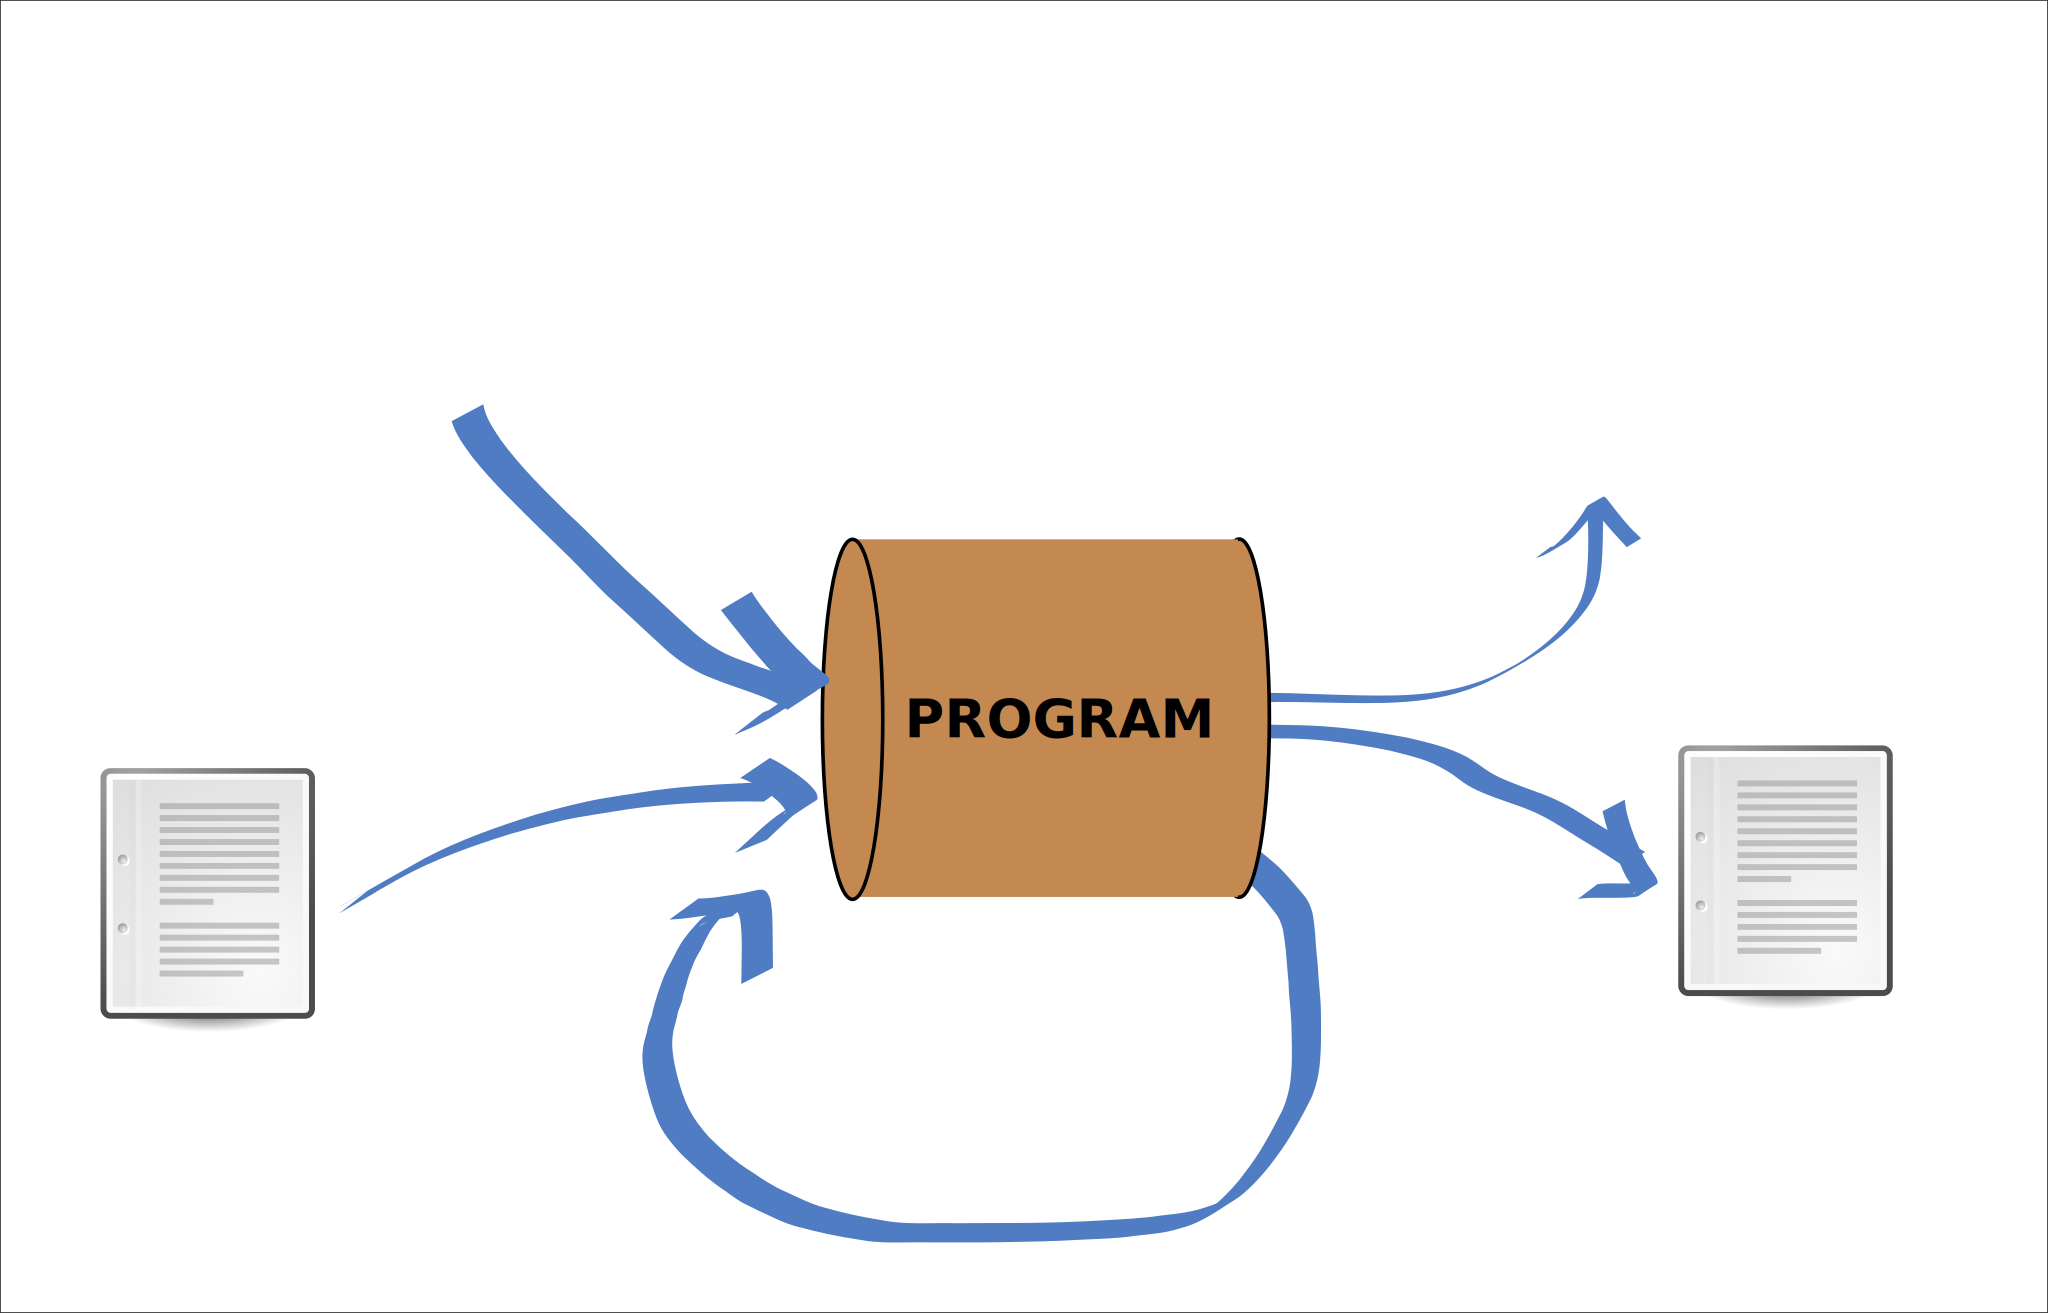
\includegraphics[scale=.15]{linux03.ps}
\end{figure}
\end{frame}


\begin{frame}[fragile]
\begin{lstlisting}[language=bash]
$ programname (options) (files)
\end{lstlisting}
\end{frame}

\begin{frame}[fragile]
\frametitle{Navigation}

where am I ?
\begin{lstlisting}[language=bash]
$ pwd
\end{lstlisting}

Go to directory dir1
\begin{lstlisting}[language=bash]
$ cd dir1
\end{lstlisting}

Go to directory dir1/dir2
\begin{lstlisting}[language=bash]
$ cd dir1/dir2
\end{lstlisting}


Go upper directory
\begin{lstlisting}[language=bash]
$ cd ..
\end{lstlisting}

Go upper directory and then go to dir4
\begin{lstlisting}[language=bash]
$ cd ../dir4
\end{lstlisting}


\end{frame}

\begin{frame}[fragile]
\frametitle{Navigation}

Go to the root
\begin{lstlisting}[language=bash]
$ cd /
\end{lstlisting}

Go to my home
\begin{lstlisting}[language=bash]
$ cd ~
\end{lstlisting}

Go to my previous directory
\begin{lstlisting}[language=bash]
$ cd /
\end{lstlisting}

\end{frame}


\begin{frame}[fragile]
 \begin{center}
    \huge{Completion}\\
  \end{center}
\end{frame}


\begin{frame}[fragile]
 \begin{center}
    \huge{CASE matters}\\
    \end{center}
\begin{lstlisting}[language=bash]
$ cd dir1
\end{lstlisting}


\begin{lstlisting}[language=bash]
$ cd DIR1
\end{lstlisting}

\end{frame}


\begin{frame}[fragile]
Regular Expression.\\
'?' : The question mark indicates there is zero or one of the preceding element. For example, colou?r matches both "color" and "colour".\\
'*' : The asterisk indicates there is zero or more of the preceding element. For example, ab*c matches "ac", "abc", "abbc", "abbbc", and so on.\\
'+' : The plus sign indicates there is one or more of the preceding element. For example, ab+c matches "abc", "abbc", "abbbc", and so on, but not "ac".\\
(a|b)* denotes the set of all strings.\\
\[ \] : A bracket expression. Matches a single character that is contained within the brackets.\\
\^ 	Matches the starting position within the string.\\
\$ 	Matches the ending position of the string or the position just before a string-ending newline.
\end{frame}


\begin{frame}[fragile]
Escape characters.\\
Cariage Return.
\begin{lstlisting}[language=bash]
\n
\end{lstlisting}
Tabulation.
\begin{lstlisting}[language=bash]
\t
\end{lstlisting}
\end{frame}


\begin{frame}[fragile]
Shell shortcuts.\\
Arrow-up/down: prev/next in history.\\
Ctr-R : Search history.\\
Ctr-A : Begin line.\\
Ctr-E : End line.\\
Ctr-K : Cut line.\\
Ctr-D and tab : insert tabulation.\\
Ctr-D and tab : insert tabulation.\\
Ctr-D (in pipeline): EOF (End Of File).\\
\end{frame}


\begin{frame}[fragile]
 \begin{center}
    \huge{whitespaces matter}\\
    \end{center}
\begin{lstlisting}[language=bash]
$ cd my results
bash: cd: my: No such file or directory
\end{lstlisting}


\begin{lstlisting}[language=bash]
$ cd  "my results"
\end{lstlisting}

\begin{lstlisting}[language=bash]
$ cd my\ results
\end{lstlisting}
  
\end{frame}





\begin{frame}[fragile]
 \begin{center}
    \huge{man}\\
    \end{center}
\begin{lstlisting}[language=bash]
$ man man

MAN(1)                                                               

NAME
       man - an interface to the on-line reference

SYNOPSIS
       man  [-C  file]  [-d]  [-D]  [--warnings[=wa
       [--names-only] [-a] [-u] [--no-subpages] [-P 
       [-X[dpi]] [-Z] [[section] page ...] ...
       man -k [apropos options] regexp ...
       man -K [-w|-W] [-S list] [-i|-I] [--regex] [s
       man -f [whatis options] page ...
       man  -l  [-C  file]  [-d]  [-D] [--warnings[=w
       man -w|-W [-C file] [-d] [-D] page ...
       man -c [-C file] [-d] [-D] page ...

\end{lstlisting}
\end{frame}


\begin{frame}[fragile]
 \begin{center}
    \huge{apropos}\\
    \end{center}
\begin{lstlisting}[language=bash]
$ apropos apropos
apropos (1)          - search the manual page names and 

$ apropos pdf
pdfcrop (1)          - crop pdf files to their minimal 
a2ping (1)           - - convert between PS, EPS and PD
dvipdf (1)           - Convert TeX DVI file to PDF usin
dvipdfm (1)          - Produce PDF files directly from
dvipdft (1)          - create thumbnail images for use 
e2pall (1)           - convert all EPS files in a LaTeX
\end{lstlisting}
\end{frame}

\begin{frame}[fragile]
 \begin{center}
    \huge{pwd}\\
    \end{center}
\begin{lstlisting}[language=bash]
$ pwd
/home/lindenb/src/courses/about.linux
\end{lstlisting}
\end{frame}

\begin{frame}[fragile]
 \begin{center}
    \huge{mkdir}\\
    \end{center}
\begin{lstlisting}[language=bash]
$ mkdir DIR1
$ mkdir DIR1/DIR2
$ mkdir -p DIR1/DIR3/DIR3
\end{lstlisting}
\end{frame}

\begin{frame}[fragile]
 \begin{center}
    \huge{ls}\\
    \end{center}
\begin{lstlisting}[language=bash]
$ ls
$ ls -l
$ ls -la
$ ls -la /home/
\end{lstlisting}
\end{frame}

\begin{frame}[fragile]
 \begin{center}
    \huge{stdin, stderr, stdout}\\
  \end{center}
\end{frame}


\begin{frame}[fragile]
 \begin{center}
    \huge{Redirection}\\
  \end{center}
\begin{lstlisting}[language=bash]
$ echo "Hello" > file1.txt
$ echo "Hello" > file1.txt
$ echo "Hello" > file1.txt
$ cat file1.txt 
Hello
\end{lstlisting}

\begin{lstlisting}[language=bash]
$ echo "Hello" >> file2.txt
$ echo "Hello" >> file2.txt
$ echo "Hello" >> file2.txt
$ cat file2.txt 
Hello
Hello
Hello
\end{lstlisting}
\end{frame}


\begin{frame}[fragile]
 \begin{center}
    \huge{Reading}\\
  \end{center}
\begin{lstlisting}[language=bash]
$ grep Hello << BARBAPAPA
> Hello
> Hello
> world
> BARBAPAPA
Hello
Hello
\end{lstlisting}
\end{frame}


\begin{frame}[fragile]
 \begin{center}
    \huge{Pipe}\\
  \end{center}
\begin{lstlisting}[language=bash]
$ gunzip -c input.vcf.gz | grep -v '#' | cut -f 1,2,3 | tr "\t" "." | sed 's/chr//' | sort -t '.'  -k2,2rn | uniq  | cat -n

     1	1.871334.rs4072383
     2	1.870903.rs13303094
     3	1.866511.rs71576583
     4	1.866319.rs9988021
     5	1.861630.rs2879816
     6	1.861008.rs28521172
     7	1.762273.rs3115849

\end{lstlisting}
\end{frame}

\begin{frame}[fragile]
 \begin{center}
    \huge{echo}\\
    \end{center}
\begin{lstlisting}[language=bash]
$ echo "ABCD"
$ echo -n "ABCD"
$ echo -e "A\tB\nCD"
\end{lstlisting}
\end{frame}

\begin{frame}[fragile]
 \begin{center}
    \huge{'file'}\\
     	Determine what type of data is within a file.\\
    \end{center}
\begin{lstlisting}[language=bash]
$ file ~/jeter.vcf.gz ~/Documents/2011028.odp
/home/lindenb/jeter.vcf.gz:          gzip compressed data, extra field
/home/lindenb/Documents/2011028.odp: OpenDocument Presentation
\end{lstlisting}
\end{frame}


\begin{frame}[fragile]
 \begin{center}
    \huge{'tr'}\\
     	translate or delete characters.\\
    \end{center}
\begin{lstlisting}[language=bash]
$ echo "AAAAAAABCD" | tr "A" "a"
aaaaaaaBCD

$ echo "AAAAAAABCD" | tr -s "A" 
ABCD

$ echo "AAAAAAABCD" | tr -d "A" 
BCD
\end{lstlisting}
\end{frame}

\begin{frame}[fragile]
 \begin{center}
    \huge{rm}\\
    \end{center}
\begin{lstlisting}[language=bash]
$ rm file1.txt file2.txt
$ rm -r DIR1/file1.txt
$ rm -i DIR1/file1.txt
$ rm -f DIR1/file1.txt
\end{lstlisting}
\end{frame}



\begin{frame}[fragile]
 \begin{center}
    \huge{rmdir}\\
    \end{center}
\begin{lstlisting}[language=bash]
$ rmdir DIR1
\end{lstlisting}
\end{frame}

\begin{frame}[fragile]
 \begin{center}
    \huge{mv}\\
    \end{center}
\begin{lstlisting}[language=bash]
$ mv DIR1/file1.txt DIR2/
$ mv olname.txt newname.txt
\end{lstlisting}
\end{frame}


\begin{frame}[fragile]
 \begin{center}
    \huge{cp}\\
    \end{center}
\begin{lstlisting}[language=bash]
$ cp olname.txt newname.txt
\end{lstlisting}
\end{frame}



\begin{frame}[fragile]
 \begin{center}
    \huge{more}\\
    \end{center}
\begin{lstlisting}[language=bash]
$ more file1.txt file2.txt
\end{lstlisting}
\end{frame}





\begin{frame}[fragile]
 \begin{center}
    \huge{cat}\\
    \end{center}
\begin{lstlisting}[language=bash]
$ cat file1.txt file2.txt
$ cat -n file1.txt
\end{lstlisting}
\end{frame}


\begin{frame}[fragile]
 \begin{center}
    \huge{head}\\
     output the first part of files.\\
    \end{center}
\begin{lstlisting}[language=bash]
$ head file1.txt
$ head -n 100 file1.txt
\end{lstlisting}
\end{frame}


\begin{frame}[fragile]
 \begin{center}
    \huge{tail}\\
     output the last part of files.\\
    \end{center}
\begin{lstlisting}[language=bash]
$ head file1.txt
$ head -n 100 file1.txt
\end{lstlisting}
\end{frame}



\begin{frame}[fragile]
 \begin{center}
    \huge{grep}\\
    \end{center}
\begin{lstlisting}[language=bash]
$ grep Gene1 genes.txt
$ grep -v Gene1 genes.txt
$ grep -i Gene1 genes.txt
$ grep -E '(Gene1|Protein1)' genes.txt
\end{lstlisting}
\end{frame}


\begin{frame}[fragile]
 \begin{center}
    \huge{cut}\\
    \end{center}
\begin{lstlisting}[language=bash]
$ cut -d '	' -f1,2,4-10 file1
$ cut -c1-10 file1
\end{lstlisting}
\end{frame}

\begin{frame}[fragile]
 \begin{center}
    \huge{sort}\\
    \end{center}
\begin{lstlisting}[language=bash]
$ sort file 
\end{lstlisting}
\end{frame}


\begin{frame}[fragile]
 \begin{center}
    \huge{nano}\\
    \end{center}
\end{frame}


\begin{frame}[fragile]
 \begin{center}
    \huge{uniq}\\
    \end{center}
\begin{lstlisting}[language=bash]
$ sort file | uniq
$ sort file | uniq -u
$ sort file | uniq -d
\end{lstlisting}
\end{frame}


\begin{frame}[fragile]
 \begin{center}
    \huge{wc}\\
    \end{center}
\begin{lstlisting}[language=bash]
$ wc file
\end{lstlisting}
\end{frame}


\begin{frame}[fragile]
 \begin{center}
    \huge{awk for filtering}\\
    \end{center}
\begin{lstlisting}[language=bash]
awk -F '	' '($1=="chr1" && int($2)>10 && int($2)<100)' file.vcf
\end{lstlisting}
\end{frame}

\begin{frame}[fragile]
 \begin{center}
    \huge{join}\\
    \end{center}
\begin{lstlisting}[language=bash]
$ join -t '	' -1 1 -2 1 file1.txt file2.txt
\end{lstlisting}
\end{frame}

\begin{frame}[fragile]
 \begin{center}
    \huge{comm}\\
    \end{center}
\begin{lstlisting}[language=bash]
$ comm file1.txt file2.txt
$ comm -12 file1.txt file2.txt
\end{lstlisting}
\end{frame}


\begin{frame}[fragile]
 \begin{center}
    \huge{gzip , gunzip}\\
    \end{center}
\begin{lstlisting}[language=bash]
$ gzip file1.txt
$ gunzip -c file1.txt.gz
$ gunzip  file1.txt
\end{lstlisting}
\end{frame}

\begin{frame}[fragile]
\begin{center}
    \huge{sed}\\
\end{center}
Usage:
\begin{lstlisting}[language=make]
sed 's/PATTERN/REPLACEBY/MODIFIER'
\end{lstlisting}
Examples:
\begin{lstlisting}[language=make]
$ echo "chr1 chr2 chr3" | sed 's/chr/CHROM_/'
CHROM_1 chr2 chr3
$ echo "chr1 chr2 chr3" | sed 's/chr/CHROM_/g'
CHROM_1 CHROM_2 CHROM_3
$ echo "chr1 chr2 chr3" | sed 's/Chr/CHROM_/gi'
CHROM_1 CHROM_2 CHROM_3
$ echo "chr1 chr2 chr3" | sed 's/chr/CHROM_/2'
chr1 CHROM_2 chr3
\end{lstlisting}
\end{frame}


\begin{frame}[fragile]
 \begin{center}
    \huge{cmp}\\
    \end{center}
\begin{lstlisting}[language=bash]
$ cmp file1 file2
\end{lstlisting}
\end{frame}

\begin{frame}[fragile]
 \begin{center}
    \huge{diff}\\
    \end{center}
\begin{lstlisting}[language=bash]
$ diff file1 file2
\end{lstlisting}
\end{frame}

\begin{frame}[fragile]
 \begin{center}
    \huge{find}\\
    \end{center}
\begin{lstlisting}[language=bash]
$ find /path1 /path2/dir2 -name "*.vcf.gz"
\end{lstlisting}
\end{frame}

\begin{frame}[fragile]
 \begin{center}
    \huge{paste}\\
    \end{center}
\begin{lstlisting}[language=bash]
$ paste file1 file2 file3 file4
\end{lstlisting}
\end{frame}

\begin{frame}[fragile]
 \begin{center}
    \huge{curl}\\
    \end{center}
\begin{lstlisting}[language=bash,breaklines=true]
$  curl "ftp://ftp.1000genomes.ebi.ac.uk/vol1/ftp/release/20110521/ALL.wgs.phase1_release_v3.20101123.snps_indels_sv.sites.vcf.gz" |\
   gunzip -c | head
   
##fileformat=VCFv4.1
##INFO=<ID=LDAF,Number=1,Type=Float,Description="MLE Allele Frequency Accounting for LD">
##INFO=<ID=AVGPOST,Number=1,Type=Float,Description="Average posterior probability from MaCH/Thunder">
##INFO=<ID=RSQ,Number=1,Type=Float,Description="Genotype imputation quality from MaCH/Thunder">
##INFO=<ID=ERATE,Number=1,Type=Float,Description="Per-marker Mutation rate from MaCH/Thunder">
##INFO=<ID=THETA,Number=1,Type=Float,Description="Per-marker Transition rate from MaCH/Thunder">
##INFO=<ID=CIEND,Number=2,Type=Integer,Description="Confidence interval around END for imprecise variants">
##INFO=<ID=CIPOS,Number=2,Type=Integer,Description="Confidence interval around POS for imprecise variants">
##INFO=<ID=END,Number=1,Type=Integer,Description="End position of the variant described in this record">
##INFO=<ID=HOMLEN,Number=.,Type=Integer,Description="Length of base pair identical micro-homology at event breakpoints">
\end{lstlisting}
\end{frame}

\begin{frame}[fragile]
 \begin{center}
    \huge{curl + NCBI}\\
    \end{center}
\begin{lstlisting}[language=bash]
$ curl -sg 'http://www.ncbi.nlm.nih.gov/entrez/eutils/esearch.fcgi?db=pubmed&term=watson[AU]+crick[AU]+1953[Date+-+Publication]'  
<?xml version="1.0" encoding="UTF-8"?>
<eSearchResult>
  <Count>3</Count>
  <RetMax>3</RetMax>
  <RetStart>0</RetStart>
  <IdList>
    <Id>13063483</Id>
    <Id>13054692</Id>
    <Id>13168976</Id>
  </IdList>
 \end{lstlisting}
\end{frame} 


\begin{frame}[fragile]
 \begin{center}
    \huge{curl + NCBI}\\
    \end{center}
\begin{lstlisting}[language=bash,breaklines=true]
$ curl -sg 'http://www.ncbi.nlm.nih.gov/entrez/eutils/efetch.fcgi?db=pubmed&id=13063483,13054692,13168976&retmode=xml' |\
grep ArticleTitle

<ArticleTitle>Genetical implications of the structure of deoxyribonucleic acid.</ArticleTitle>
<ArticleTitle>Molecular structure of nucleic acids; a structure for deoxyribose nucleic acid.</ArticleTitle>
<ArticleTitle>The structure of DNA.</ArticleTitle>
 \end{lstlisting}
\end{frame} 

\begin{frame}[fragile]
 \begin{center}
    \huge{script}\\
    \end{center}
\begin{lstlisting}[language=bash,breaklines=true]
$ script myfile.txt
Script started, file is myfile.txt
$ echo "Hello"
Hello
$ exit
Script done, file is myfile.txt
$ cat myfile.txt 

> Script started on Thu 25 Jun 2015 11:50:43 AM CEST
> $ echo "Hello"
> Hello
> $ exit
> Script done on Thu 25 Jun 2015 11:50:52 AM CEST

 \end{lstlisting}
\end{frame} 


\begin{frame}[fragile]
 \begin{center}
    \huge{bc}\\
  \end{center}
\begin{lstlisting}[language=bash]
$ echo "(13.3*2)/2.3" | bc
11
$ echo "(13.3*2)/2.3" | bc -l
11.56521739130434782608
\end{lstlisting}
\end{frame}



\begin{frame}[fragile]
 \begin{center}
    \huge{chown/chmod/chgrp}\\
    \end{center}
\begin{lstlisting}[language=bash,breaklines=true]
chown pierre file.txt
chgrp bioinformatics file.txt
chmod u+rw file.txt
chmod g+r file.txt
\end{lstlisting}
\end{frame} 

\begin{frame}[fragile]
\begin{center}
    \huge{sqlite3}\\
    \end{center}
\begin{lstlisting}[language=bash]  
$ sqlite3 test.sqlite3
SQLite version 3.7.9 2011-11-01 00:52:41
Enter ".help" for instructions
Enter SQL statements terminated with a ";"
sqlite> create table Person(name text);
sqlite> insert into Person(name) values('Pierre');
sqlite> insert into Person(name) values('Paul');
sqlite> insert into Person(name) values('Jacques');
sqlite> select name from Person;
Pierre
Paul
Jacques
\end{lstlisting}
\end{frame}



\begin{frame}[fragile]
\begin{center}
    \huge{mysql}\\
    \end{center}
\begin{lstlisting}[language=bash,breaklines=true]  
$ mysql --user=genome --host=genome-mysql.cse.ucsc.edu -D hg19 -e 'select chrom,chromStart,chromEnd,Observed from snp141 where name="rs25"'
+-------+------------+----------+----------+
| chrom | chromStart | chromEnd | Observed |
+-------+------------+----------+----------+
| chr7  |   11584141 | 11584142 | A/G      |
+-------+------------+----------+----------+
\end{lstlisting}
\end{frame}


\begin{frame}[fragile]
 \begin{center}
    \huge{R}\\
    \end{center}
\begin{lstlisting}
SampleID	Dye	Concentration1l	Concentration2	rapp	Qt	AS	Vol
E1-4	Cy5	3,52	203,79	2,25	6,1	17,3	4,05
E1-5	Cy3	3,14	174,16	2,22	5,2	18	4,74
E2-4	Cy3	1,64	101,18	2,25	3	16,2	8,15
E2-5	Cy3	3,41	213,74	2,26	6,4	16	3,86
E3-4	Cy3	3,11	184,15	2,22	5,5	16,9	4,48
E3-5	Cy5	3,58	189,31	2,24	5,7	18,9	4,36
mean(samples$Concentration2)
\end{lstlisting}
\begin{lstlisting}[language=R]
    samples <- read.table("samples2.txt",
    	dec=",",
    	header=TRUE)
mean(samples$Concentration2)
\end{lstlisting}
\end{frame}


\begin{frame}[fragile]
 \begin{center}
    \huge{'git'}\\
    \end{center}
\begin{lstlisting}[basicstyle=\tiny]
mkdir test
cd test
git init
Initialized empty Git repository in test/.git/
$ git add  file.txt
$ git commit -m "Added one file"
[master (root-commit) 4954d33] Added one file
$ echo "World" >> file.txt
$ git diff
diff --git a/file.txt b/file.txt
@@ -1 +1,2 @@
 Hello
+World
$ git add  file.txt
$ git commit -m "added hello"
$ git log file.txt
(...)
$ git rm file.txt
$ git checkout file.txt
\end{lstlisting}
\end{frame}

\begin{frame}[fragile]
 \begin{center}
    \huge{'LaTeX'}\\
  \end{center}
\begin{verbatim}
\documentclass{article}
\title{My Thesis}
\author{Pierre}
\date{September 2015}
\begin{document}
   \maketitle
   Hello world!
\end{document}
\end{verbatim}

\begin{lstlisting}[language=bash]
pdflatex input.tex
\end{lstlisting}  
\end{frame}

\begin{frame}[fragile]
 \begin{center}
    \huge{Install a program}\\
  \end{center}
\begin{lstlisting}[language=bash]
curl -kL -o bwa-0.7.12.zip -L "https://github.com/lh3/bwa/archive/0.7.12.zip"
unzip bwa-0.7.12.zip
make -C bwa-0.7.12/
\end{lstlisting}  
\end{frame}


\begin{frame}[fragile]
 \begin{center}
    \huge{bash Scripting}\\
  \end{center}
\end{frame}

\begin{frame}[fragile]
 \begin{center}
    \huge{chmod+x and shebang}\\
  \end{center}
\end{frame}



\begin{frame}[fragile]
 \begin{center}
    \huge{bash script}\\
    \end{center}
\begin{lstlisting}[language=bash]
#!/bin/bash
echo "Hello " > hello.txt
echo "World" > world.txt
cat hello.txt world.txt > hellodworld.txt
\end{lstlisting}
\end{frame}




\begin{frame}[fragile]
 \begin{center}
    \huge{make}\\
    \end{center}
\begin{lstlisting}[language=bash]
#!/bin/bash 
function quit {
   exit
}  
function e {
    echo $1 
}  
e Hello
e World
quit
echo foo 
\end{lstlisting}
\end{frame}


\begin{frame}[fragile]
 \begin{center}
    \huge{Simple math}\\
    \end{center}
\begin{lstlisting}[language=bash]
echo $((1+1)) 
\end{lstlisting}
\end{frame}

\begin{frame}[fragile]
 \begin{center}
    \huge{Simple math}\\
    \end{center}
\begin{lstlisting}[language=bash]
#!/bin/bash
for i in 1 2 3 4 5 6; do
    echo item: $i
done
\end{lstlisting}
\end{frame}

\begin{frame}[fragile]
 \begin{center}
    \huge{While read}\\
    \end{center}
\begin{lstlisting}[language=bash]
#!/bin/bash
cat file.txt | while read L; do
    echo $L
done
\end{lstlisting}
\end{frame}

\begin{frame}[fragile]
 \begin{center}
    \huge{Make Scripting}\\
  \end{center}
\end{frame}


\begin{frame}[fragile]
 \begin{center}
    \huge{make}\\
    \end{center}
\begin{lstlisting}[language=make]
all: hellodworld.txt
        cat $<
hellodworld.txt: hello.txt world.txt
        cat $^ > $@
hello.txt:
        echo "Hello " > $@
world.txt:
        echo "World" > $@
clean:
        rm -f hellodworld.txt  hello.txt world.txt
\end{lstlisting}
\end{frame}


\begin{frame}[fragile]
See  also: 
\begin{itemize}
\item \url{http://korflab.ucdavis.edu/Unix\_and\_Perl/current.html}
\item \url{http://unix.stackexchange.com/}
\item \url{http://stackoverflow.com/}
\item \url{https://www.biostars.org/}
\end{itemize}
\end{frame}

\end{document}

